\section{内存存储策略}

AI应用具有数据访问和通信密集型的特点,内存访问效率与处理器运行速度的差异引发了存储墙问题,使得内存访问和通信成为性能瓶颈。

在Chiplet架构中,由于多芯粒功能划分,不会引入各个功能组件内部架构的新问题,而是需要重点考虑和解决跨芯粒所产生的问题,包括芯片互连架构和软件架构的变化。
下面以基于UCIe(Universal Chiplet Interconnect Express, 通用小芯片快连)的M.link结构为例,介绍常用的内存存储策略。

\subsection{基于UCIe的M.link的内存存储层次结构}

下图8显示了 M.Link 的层次结构,它由主结构层和次结构层、协议层、链路层和物理层组成。由于 UCIe™ 仅指定链路层和物理层支持标准和高级包的每个模块 16 和 64 个通道,因此在 M.Link 中为 D2D 接口定义了额外的层。内存控制和链路之间的结构层和协议层应支持在几纳秒的短延迟内进行数据流控制和格式转换,以降低带宽损失。M.Link 模块设计有 16 个通道,数据速率高达8GT/s,支持高达 16GBps/模块 $\texttt{\cite{Sharma2020PCIe6}}$,并且可以通过添加更多模块来增加总带宽。为了补偿时钟和数据通道之间的偏差并实现高达 10e-15 的 BER(误码率)要求,实施了使用 DLL(延迟锁定环)和 LSFR(线性反馈移位寄存器)模式的位线偏差控制和时钟训练方案。

\begin{figure}[htbp]
	\centering
	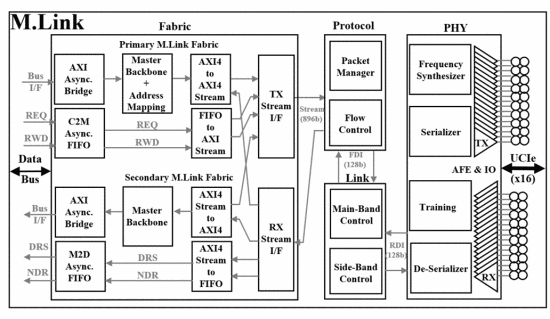
\includegraphics[width=0.6\textwidth]{img/4-1.png} % 图片文件名,不需要加扩展名
	\caption{基于UCIe™标准的M.Link框图 \cite{10848977}}
	\label{fig:example}
\end{figure}

\subsection{以M.Link为例的时钟方案}
图9中,有三种用于多芯片参考时钟的方案。使用外部晶振或内部振荡器等参考时钟源时,工作频率没有偏移。然而,第一种方案需要在电路板上增加元件,成本较高;第二种方案需要为主控制器的前向时钟提供一个I/O,功耗较大。

另一种方案在每个芯片中使用内部振荡器作为独立的参考时钟,可能会产生频率偏移。如果主控制器(快速 CLK2)的工作频率比次控制器(慢速CLK2)快,则由于吞吐量差异,次控制器的接收器无法完全恢复数据。为了保持接收器的有效带宽大于发射器的有效带宽,M.Link 使用减慢缓冲区来控制数据流,即在传输数据的中间添加一些空闲状态。尽管这会降低数据带宽,但是能极大地降低成本和提高模块组装灵活性。

\begin{figure}[htbp]
	\centering
	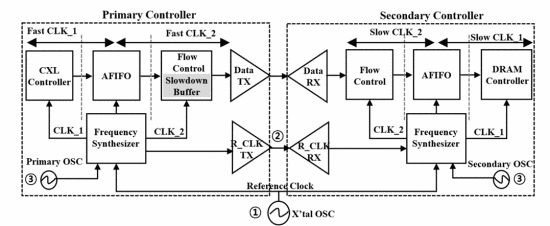
\includegraphics[width=0.6\textwidth]{img/4-2.png} % 图片文件名,不需要加扩展名
	\caption{M.Link的参考时钟方案 \cite{10848977}}
	\label{fig:example}
\end{figure}